\documentclass[a4paper,12pt]{article}

\usepackage[french]{babel}
\usepackage[utf8]{inputenc}
\usepackage{graphicx}
\usepackage{array}
\usepackage{multirow}
\usepackage{hyperref}
\usepackage{lscape}
\hypersetup{colorlinks, citecolor=black, filecolor=black, linkcolor=black, urlcolor=black}

\title{Cahier des charges du Projet Nigma}
\author{CrypTeam : LAPÔTRE Guillaume (\texttt{lapotr\_g}) \and GANIVET Justin (\texttt{ganive\_j}) \and LADEVIE Stéphane (\texttt{ladevi\_s}) \and GISLAIS Sébastien (\texttt{gislai\_s})}
\pagestyle{myheadings}
\date{21 novembre 2008}

\begin{document}
\markright{Cahier des charges de la CrypTeam}
\maketitle{}
\newpage
\tableofcontents
\newpage
\part{Introduction}
%introduction rapide

\section {Présentation de la CrypTeam}

\section {Présentation individuelle}

\subsection{Guillaume LAPÔTRE}

Actuellement étudiant en Info-spé à EPITA, j'entame avec réjouissance ce fabuleux projet à la fois utile et pédagogique. En effet, la cryptographie m'a toujours attiré. Mais je n'ai jamais eut l'occasion de m'y interressé de plus près. La stéganographie n'était pas mon idée mais je l'ai trouvé assez interressante. Ainsi je pourrais découvrir des principes algorithmiques pour chiffrer et déchiffrer des messages puis les cacher dans une image !

\subsection{Justin GANIVET}

\subsection{Stéphane LADEVIE}

\subsection{Sébastien GISLAIS}

\newpage

\part{\'{E}tat de l'art}
La cryptographie et la stéganographie sont deux techniques extrêmement anciennes permettant de transmettre des informations uniquement aux personnes voulues.

La cryptographie protège le message en le chiffrant, c'est-à-dire en le rendant incompréhensible sans connaître l'algorithme de cryptage. On peut citer comme procédé de cryptage historique le chiffre de César qui décale l'alphabet de $n$ rang suivant le chiffre choisi (ainsi si le chiffre choisi est 3, l'alphabet sera : DEFGHI\dots{}ZABC).

La stéganographie consiste à cacher le message à transmettre plutot que de le chiffrer. Comme exemple historique, on peut citer un procédé utilisé par César : il écrivait sur le crâne d'un esclave un message puis attendait que les cheveux de cet esclave repoussent. Il envoyait ensuite l'esclave à la personne à qui le message était destiné. Il suffisait donc de raser l'esclave pour récupérer le message.

Cependant, la stéganographie ainsi que la cryptographie étaient utilisées quasiment uniquement par les militaires avant la fin de la Seconde Guerre Mondiale. Depuis, il y a énormément d'application civile au chiffrement.

\section{Cryptographie}

\subsection{Cryptage par substitution}

Le cryptage par substitution est une des techniques les plus basique et les plus ancienne de chiffrement. Le chiffre de César est une technique de cryptage par substitution. Il existe plusieurs types de substitution pour chiffrer des données.

\subsubsection{Le cryptage par substitution mono-alphabétique}

On remplace chaque lettres de l'alphabet par une autre lettre. Ainsi pour la première lettre il y a 26 possibilités, pour la seconde 25 possibilités, etc. Il existe donc $26!$ façons distinctes de coder. L'inconvénient de la substitution mono-alphabétique est qu'il faut se souvenir de chaque substitution pour chaque lettre. L'autre inconvénient est qu'en connaissant la langue du message codé on peut relativement facilement déchiffrer le message en se basant sur la fréquence d'apparition de chaque lettre dans la langue. Par exemple en français la lettre apparaissant le plus souvent est le E. En analysant un texte chiffré avec cette technique de chiffrement, on peut trouver la lettre qui apparaît le plus souvent et l'associer donc à la lettre E. Ensuite on utilise le même raisonnement pour toutes les autres lettres.

\subsubsection{Le codage par substitution poly-alphabétique}

Le chiffre de Vigenère est un bon exemple de codage par substitution poly-alphabétique. On crée un mot qui sert de clé et on le \og colle \fg{} en dessous du texte à chiffrer. Pour chiffrer ou déchiffrer un message on utilise une matrice $26 \times 26$ avec l'alphabet sur la première ligne et sur la première colonne. Ensuite, on crypte chaque lettre à l'aide de la lettre de la clé que l'on a disposée juste en dessous avec la matrice ci-dessous.

\begin{center}
  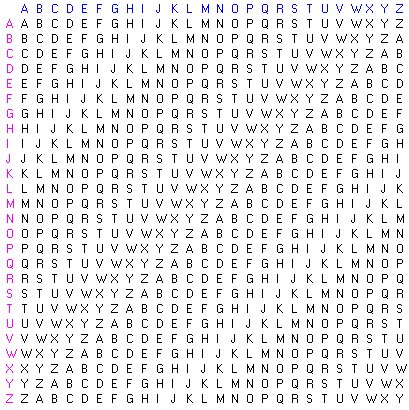
\includegraphics[scale=0.5]{../Image/matrice.jpg}
  % matrice.jpg: 409x410 pixel, 72dpi, 14.43x14.46 cm, bb=0 0 409 410
\end{center}

Exemple : Chiffrons le mot \texttt{Poney} à l'aide de la clé \texttt{EPITA} :\\
\texttt{Poney}\\
\texttt{EPITA}\\
\texttt{Poney} chiffré avec cette clé :
\begin{itemize}
\item P crypté avec la lettre E : T
\item O crypté avec la lettre P : D
\item N crypté avec la lettre I : V
\item E crypté avec la lettre T : X
\item Y crypté avec la lettre A : Y
\end{itemize}
\texttt{Poney} crypté à l'aide de la clé \texttt{EPITA} avec le chiffre de Vigenère donne \texttt{TDVXY} !

\subsection{Cryptage symétrique}

\subsubsection{DES (\emph{Data Encryption Standard})}

Jusque dans les années 1970, seuls les militaires possédaient des algorithmes à clé secrète fiables. Devant l'émergence de besoins civils, le NBS (\emph{National Bureau of Standards}) lança le 15 mai 1973 un appel d'offres dans le \emph{Federal Register} (l'équivalent du \emph{Journal Officiel} américain) pour la création d'un système cryptographique. Le cahier des charges était le suivant :

\begin{itemize}
\item l'algorithme repose sur une clé relativement petite, qui sert à la fois au chiffrement et au déchiffrement
\item l'algorithme doit être facile à implémenter, logiciellement et matériel\-lement, et doit être très rapide
\item le chiffrement doit avoir un haut niveau de sûreté, uniquement lié à la clé, et non à la confidentialité de l'algorithme
\end{itemize}

Les efforts conjoints d'IBM, qui propose l'algorithme \emph{Lucifer} fin 1974, et de la NSA (\emph{National Security Agency}) conduisent à l'élaboration du DES (\emph{Data Encryption Standard}), l'algorithme de chiffrement le plus utilisé au monde durant le dernier quart du XX\ieme{} siècle.

La clé du DES est une chaîne de 64 bits, mais en fait seuls 56 bits servent réellement à définir la clé. Les bits 8, 16, 24, 32, 40, 48, 56 et 64 sont des bits de parité (bits de détection d'erreur). Le 8\ieme{} bit est fait en sorte que sur les 8 premiers bits, il y ait un nombre impair de 1. Par exemple, si les 7 premiers bits sont 1010001, le 8\ieme{} bit est 0. Ceci permet d'éviter les erreurs de transmission.

Il y a donc pour le DES $2^{56}$ clés possibles, soit environ\dots{} 72 millions de milliards possibilités. Les grandes lignes de l'algorithme sont :

\begin{description}
\item[Phase 1 : Préparation -- Diversification de la clé.] Le texte est décou\-pé en blocs de 64 bits. On diversifie aussi la clé $K$, c'est-à-dire qu'on fabrique à partir de $K$ 16 sous-clés $K_{1}, \dots{}, K_{16}$ à 48 bits. Les $K_{i}$ sont composés de 48 bits de $K$, pris dans un certain ordre.
\item[Phase 2 : Permutation initiale.] Pour chaque bloc de 64 bits $x$ du texte, on calcule une permutation finie $y=P(x)$. $y$ est représenté sous la forme $y=G0D0$, $G0$ étant les 32 bits à gauche de $y$, $D0$ les 32 bits à droite.
\item[Phase 3 : Itération.] On applique 16 rondes d'une même fonction. A partir de $G_{i-1}D_{i-1}$ (pour $i$ de 1 à 16), on calcule $G_{i}D_{i}$ en posant :
  \begin{itemize}
  \item $G_{i} = D_{i-1}$
  \item $D_{i-1} = G_{i-1} \textrm{ XOR } f(D_{i-1},K_{i})$
  \end{itemize}
  XOR est le OU Exclusif bit à bit, et $f$ est une fonction de confusion, suite de substitutions et de permutations.
\item[Phase 4 : Permutation finale.] On applique à $G_{16}D_{16}$ l'inverse de la permutation initiale. $Z = P^{-1}(G_{16}D_{16})$ est le bloc de 64 bits chiffré à partir de $x$.
\end{description}

\begin{center}
  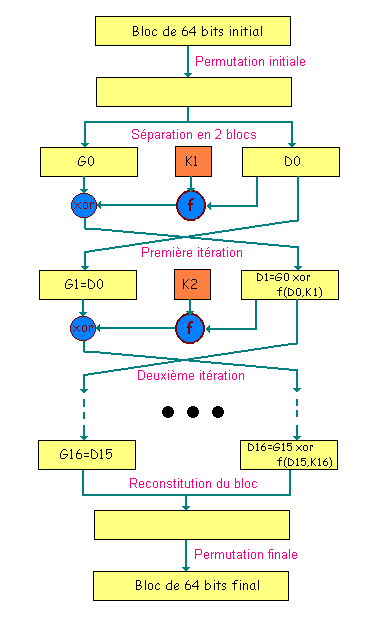
\includegraphics[scale=0.5]{../Image/des.png}
  % des2.png: 382x620 pixel, 72dpi, 13.48x21.87 cm, bb=0 0 382 620
\end{center}


Régulièrement, le DES a fait l'objet de polémiques. Toute sa sécurité repose sur la fonction de confusion $f$, et en particulier à l'intérieur de celle-ci sur des boîtes S, tableau $4 \times 16$ d'entiers compris entre 0 et 15, aux valeurs mystérieuses. Certains ont affirmé que la NSA, qui a finalisé l'algorithme, a placé dans ces boîtes S des trappes qui lui permettaient de tout décrypter, tout en affirmant que l'algorithme est sûr. Toutefois, rien n'a objectivement étayé cela. En particulier, le DES a toujours résisté aux travaux des cryptanalystes non basés sur la force brute.

En revanche, ce qui a signé l'arrêt de mort du DES est l'extraordinaire progression de la puissance des ordinateurs. Le 17 juin 1997, le DES est cassé en 3 semaines par une fédération de petites machines sur Internet. Et on estime très officiellement (dans un rapport présenté au Sénat Américain) à cette date à quelques secondes le temps nécessaire à un Etat pour percer les secrets d'un message chiffré avec le DES.

La solution a été dans un premier temps l'adoption du triple DES, trois applications de DES à la suite avec 2 clés différentes (d'où une clé de 112 bits) :

\begin{center}
  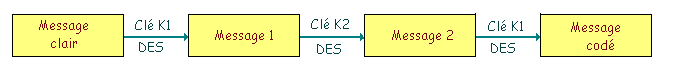
\includegraphics[width=\textwidth]{../Image/3des.png}
  % des3.png: 676x71 pixel, 72dpi, 23.85x2.50 cm, bb=0 0 676 71
\end{center}

Si le 3DES est largement suffisant à l'heure actuelle, il est malheureusement trois fois plus lent que le DES. C'est pourquoi, en janvier 1997, le NIST (\emph{National Institute of Standards and Technologies}) lance un nouvel appel pour créer un successeur au DES. L'histoire commence pour l'AES (\emph{Advanced Encryption Standard}).

\subsubsection{AES (\emph{Advanced Encryption Standard})}

Avec le temps et les progrès de l'informatique, les $2^{56}$ clés possibles du DES n'ont plus représenté une barrière infranchissable. Il est désormais possible, même avec des moyens modestes, de percer les messages chiffrés par DES en un temps raisonnable. En janvier 1997, le NIST (\emph{National Institute of Standards and Technologies}) des \'{E}tats-Unis lance un appel d'offres pour élaborer l'AES, \emph{Advanced Encryption System}. Le cahier des charges comportait les points suivants :

\begin{itemize}
\item évidemment, une grande sécurité
\item une large portabibilité : l'algorithme devant remplacer le DES, il est destiné à servir aussi bien dans les cartes à puces, aux processeurs 8 bits peu puissants, que dans des processeurs spécialisés pour chiffrer des miliers de télécommunications à la volée
\item la rapidité
\item une lecture facile de l'algorithme, puisqu'il est destiné à être rendu public
\item techniquement, le chiffrement doit se faire par blocs de 128 bits, les clés comportant 128, 192 ou 256 bits
\end{itemize}

Au 15 juin 1998, date de la fin des candidatures, 21 projets ont été déposés. Certains sont l'\oe{}uvre d'entreprises (IBM), d'autres regroupent des universitaires (CNRS), les derniers sont écrits par à peine quelques personnes. Pendant deux ans, les algorithmes ont été évalués par des experts, avec forum de discussion sur Internet, et organisation de conférences. Le 2 octobre 2000, le NIST donne sa réponse : c'est le \emph{Rijndael} qui est choisi, un algorithme mis au point par 2 belges, Vincent \textsc{Rijmen} et Joan \textsc{Daemen}.

Le \emph{Rijndael} procède par blocs de 128 bits, avec une clé de 128 bits également. Chaque bloc subit une séquence de 5 transformations répétées 10 fois :

\begin{enumerate}
\item Addition de la clé secrète (par un OU Exclusif)
\item Transformation non linéaire d'octets : les 128 bits sont répartis en 16 blocs de 8 bits (un octet !), eux-même dispatchés dans un tableau $4 \times 4$. Chaque octet est transformé par une fonction non linéaire S
\item Décalage de lignes : les 3 dernières lignes sont décalées cycliquement vers la gauche : la 2\ieme{} ligne est décalée d'une colonne, la 3\ieme{} ligne de 2 colonnes, et la 4\ieme{} ligne de 3 colonnes
\item Brouillage des colonnes : chaque colonne est transformée par combinaisons linéaires des différents éléments de la colonne (ce qui revient à multiplier la matrice $4 \times 4$ par une autre matrice $4 \times 4$). Les calculs sur les octets de 8 bits sont réalisés dans le corps à $2^{8}$ éléments
\item Addition de la clé de tour : à chaque tour, une clé de tour est générée à partir de la clé secrète par un sous-algorithme (dit de cadencement). Cette clé de tour est ajoutée par un ou exclusif au dernier bloc obtenu
\end{enumerate}

Schéma de l'algorithme AES (ou \emph{Rijndael}) :

\begin{center}
  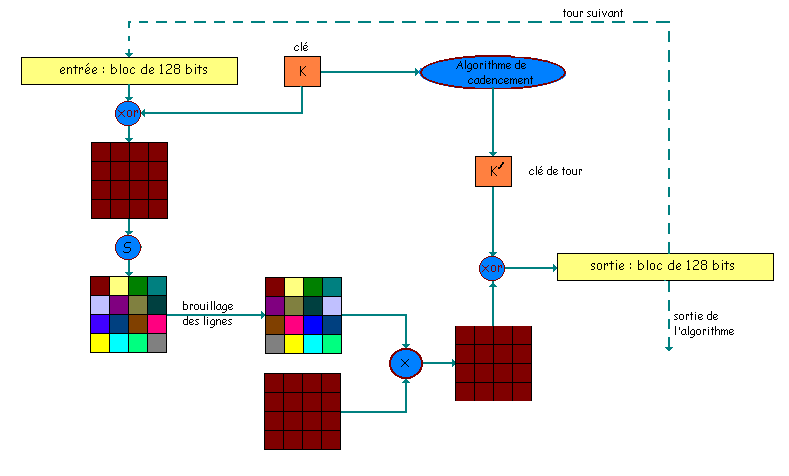
\includegraphics[width=\textwidth]{../Image/aes.png}
  % aes.png: 789x476 pixel, 72dpi, 27.83x16.79 cm, bb=0 0 789 476
\end{center}


\subsection{Cryptage asymétrique}

\subsubsection{RSA (\emph{Rivest Shamir Adleman})}

Le RSA est un algorithme méthode de cryptographie inventée en 1977 par  Ron \textsc{Rivest}, Adi \textsc{Shamir} et Len \textsc{Adleman} (d'où le nom de RSA). C'est encore le système cryptographique à clé publique le plus utilisé de nos jours.

Petite anecdote : au départ, \textsc{Rivest}, \textsc{Shamir} et \textsc{Adleman} voulaient prouver que tout système à clé plublique possède une faille, c'est ainsi qu'ils ont créé le RSA !

Son principe de fonctionnement suit 4 étapes :\\
Tout d'abord il y a la création des clés (que l'on nommera $P$, $Q$, $E$ et $D$). $P$ et $Q$ sont deux grands nombres premiers distincts. Leur génération se fait au hasard en utilisant un algorithme de test de primalité probabiliste. C'est un algorithme qui determine si un nombre est probablement premier selon le degré de probabilité que l'on a fixé dans l'algorithme. En cryptographie, on se \og contente \fg{} d'avoir un nombre dont on sait qu'il est premier avec une probabilité supérieure à $ 1 - \frac{1}{2^{100}} $. $E$ est un entier premier avec le produit $(P - 1)(Q - 1)$. $D$ est tel que $ED = 1 \textrm{ mod } (P - 1)(Q - 1)$ donc que $ED - 1$ est un multiple de $(P - 1)(Q - 1)$. On peut fabriquer $D$ à partir de $E$, $P$ et $Q$ en utilisant l'algorithme d'Euclide.

Ensuite il faut distribuer les clés. Le couple $(n, e)$ constitue la clé publique. Elle est disponible pour toute personne voulant crypter un message afin de nous l'envoyer ensuite. Le couple $(n, d)$ constitue notre clé privée que l'on garde secrète. Si une personne désire nous envoyer un message codé, elle le représente sous la forme de plusieurs entiers $M$ compris entre 0 et $n - 1$. Elle possède notre clé publique $(n, e)$ et calcule $C = M^{e} \textrm{ mod } n$. C'est ce dernier nombre qu'elle nous envoie.

Nous recevons donc $C$ et on calcule $D$ grâce à notre clé privée : $D = C^{d} \textrm{ mod } n$. D'après un théorème d'Euler $D = M^{de} = M \textrm{ mod } n$. On a donc reconstitué le message.

\section{Stéganographie}

\subsection{Stéganographie des temps anciens}

La stéganographie existe depuis des temps immemoriaux. Comme dit dans l'introduction, elle remonte jusqu'à l'époque de César ! Xeres, le roi de Perse eut aussi l'idée d'écrire sur le bois d'une tablette de cire et d'ensuite la recouvrir de cire. Ainsi la tablette semblait neuve et le message caché.

Tout le monde se souvient dans son enfance du numéro de \emph{Pif Gadget} où était expliqué le moyen de créer de l'encre sympathique. En effet, avec du jus de citron ou du lait comme encre, le message écrit devient invisible. Grâce à une bougie ou une solution chimique, on peut révéler le message secret.

\begin{center}
  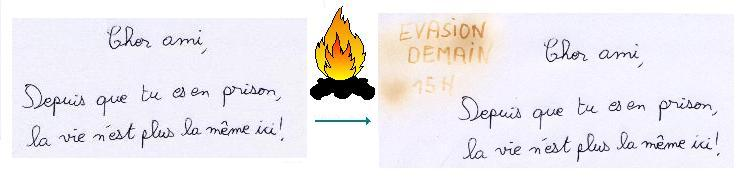
\includegraphics[width=\textwidth]{../Image/histegano1.jpg}
\end{center}

Une  autre méthode  plus littéraire est de cacher le message dans du texte. Ainsi le célèbre couple George Sand et Alfred de Musset s'est illustré lors de leurs conversations écrites. Voici le texte que George Sand envoya à Alfred de Musset :

\begin{verse}
  Cher ami,

  Je suis toute émue de vous dire que j'ai\\
  bien compris l'autre jour que vous aviez\\
  toujours une envie folle de me faire\\
  danser. Je garde le souvenir de votre\\
  baiser et je voudrais bien que ce soit\\
  une preuve que je puisse être aimée\\
  par vous. Je suis prête à montrer mon\\
  affection toute désintéressée et sans cal-\\
  cul, et si vous voulez me voir ainsi\\
  vous dévoiler, sans artifice, mon âme\\
  toute nue, daignez me faire visite,\\
  nous causerons et en amis franchement\\
  je vous prouverai que je suis la femme\\
  sincère, capable de vous offrir l'affection\\
  la plus profonde, comme la plus étroite\\
  amitié, en un mot : la meilleure épouse\\
  dont vous puissiez rêver. Puisque votre\\
  âme est libre, pensez que l'abandon ou je\\
  vis est bien long, bien dur et souvent bien\\
  insupportable. Mon chagrin est trop\\
  gros. Accourrez bien vite et venez me le\\
  faire oublier. A vous je veux me sou-\\
  mettre entièrement.

  Votre poupée
\end{verse}

Très joli n'est-ce pas ? Maintenant si vous relisez le texte une ligne sur deux vous comprendrez la vraie nature du message.

Ce à quoi Musset répondis :

\begin{verse}
  \emph{Quand} je mets à vos pieds un éternel hommage,\\
  \emph{Voulez}-vous qu'un instant je change de visage ?\\
  \emph{Vous} avez capturé les sentiments d'un c\oe{}ur\\
  \emph{Que} pour vous adorer forma le créateur.\\
  \emph{Je} vous chéris, amour, et ma plume en délire\\
  \emph{Couche} sur le papier ce que je n'ose dire.\\
  \emph{Avec} soin de mes vers lisez les premiers mots,\\
  \emph{Vous} saurez quel remède apporter à mes maux. \\
\end{verse}

Si vous lisez le premier mot de chaque vers de ce poème, vous pourrez lire la vraie réponse de Musset.

\subsection{La sténographie informatisé}

Avec l'avènement de l'informatique, et plus particulièrement avec la multiplication des transferts de fichiers sur les réseaux, la stéganographie est redevenue un sujet à la mode. Quoi de plus facile, en effet, que de glisser quelques bits discrets au milieu d'un flot d'images, de textes et de programmes. Les moyens de cacher sont innombrables, des plus rudimentaires aux plus sophistiqués.

La première méthode est de cacher le texte dans une page HTML. En effet peut importe le nombre d'espaces, le navigateur n'en affichera qu'un. Il suffit, entre les mots, d'insérer autant d'espaces que la lettre qu'on veut cacher (un espace pour A, deux espaces pour B, etc.).

Message à cacher : BIBMATHS

Description en espaces : 2-9-2-13-1-20-8-19

Une autre méthode est de cacher le message dans le disque dur sans renseigner l'index. Ainsi en ayant le numéro de l'adresse mémoire, il est possible de retrouver le message.

Mais le plus intéressant en matière de stéganographie informatique est de cacher le message dans une image. Pour le format BMP (Bitmap), chaque pixel d'une image est représenté par 3 nombres codés sur 8 bits : R représente l'intensité du rouge (un entier entre 0 et 255), G celle du vert, B celle du bleu. Si l'on modifie les 2 bits de droite de R, on modifie très peu sa valeur (au plus, de 3), et cela est imperceptible à l'\oe{}il humain. On remplace alors les 2 bits de droite de R par les 2 premiers bits du message. Puis on continue pour les composantes G, R, puis pour le 2\ieme{} pixel, etc.

\begin{center}
  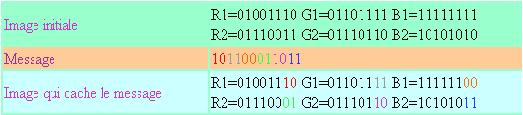
\includegraphics[width=\textwidth]{../Image/cacher_bmp.JPG}
\end{center}

Ce système est très discret puisque dans une image de $200 \times 200$ on peut cacher $200 \times 200 \times 6 = 240000$ bits, soit 30000 caractères. L'inconvénient est que la transformation en JPG perd ainsi le message.

\newpage


\part{Répartition des charges}
%descriptif précis
Nous allons coder le logiciel \emph{Nigma} qui permettra de crypter un fichier via un algorithme de cryptographie au choix puis l'incrustation dans une image par des méthodes de stéganographie. Ainsi, le fichier sera crypté puis camouflé dans une image quelconque. Il y a deux étapes importantes dans la réalisation du logiciel : le cryptage et la stéganographie. Nous considérons que les deux étapes sont liées.

Les langages de programmation que nous allons utiliser sont le \texttt{C} et le \texttt{Caml}. Notre programme sera compilé dans l'environnement Unix FreeBSD d'EPITA. Il possèdera un mode console ainsi qu'une interface graphique.

Nous allons coder la partie cryptographie majoritairement avec le langage \texttt{Caml} et la partie stéganographie majoritairement avec le langage \texttt{C}. Notre interface graphique sera quant à elle codée en \texttt{C}.

Les différentes parties de programmation sont réparties dans le groupe de la manière suivante :

\bigskip

\begin{tabular}{|l|c|c|c|c|}
  \hline
  Tâches              & Guillaume & Justin   & Stéphane & Sébastien \\ \hline \hline
  Cryptographie       & $\oplus$  &          &          & $\oplus$  \\ \hline
  Stéganographie      &           & $\oplus$ & $\oplus$ &           \\ \hline
  Interface Graphique &           & $\oplus$ & $\oplus$ &           \\ \hline
\end{tabular}


\newpage

\part{Planning de Réalisation}
%aligné sur les dates de soutenance
Pour la première soutenance, nous allons démarrer dans la partie cryptographie avec le cryptage RSA. Pour la stéganographie, nous implémenterons programme créant, à partir d'un texte, une image en niveaux de gris. Notre programme sera pour l'instant en mode console uniquement. Comme type de fichier à crypter, nous nous occuperons excusivement d'un fichier texte afin de contrôler le cryptage et le décryptage plus facilement. Nous mettrons aussi en place notre site Web, il permettra de nous présenter ainsi que notre projet. L'intégralité du code source sera disponible au téléchargement.

Pour la deuxième soutenance, nous ajouterons le cryptage DES dans la partie cryptographie. L'utilisateur aura donc le choix entre les algorithmes de cryptage RSA et DES. Du côté de la stéganographie, nous présenterons notre progression de l'intégration d'un fichier dans une image. Nous aurons une interface graphique ou une utilisation en mode console au choix pour l'utilisateur. Nous diversifierons les types de fichier à crypter en ajoutant la possibilité d'utiliser une image.

Enfin, pour la soutenance finale, nous implémenterons l'algorithme de cryptage AES que nous ajouterons aux algorithmes déjà réalisés. La partie stéganographie sera terminée, nous aurons alors notre fichier crypté qui sera incrusté dans une image. Notre interface aura sans doute évoluée au regard de notre utilisation régulière.

Tout au long du projet, notre site Web sera mis à jour et décrira l'avancée du Projet Nigma.

\bigskip

\begin{landscape}
  \begin{tabular}{|l|c|c|c|c|}
    \hline
    Soutenance & Cryptographie & Stéganographie                    & Interface        & Données d'entrée \\ \hline \hline
    1          & RSA           & création d'une image /            & mode console     & fichier texte    \\
    &               & nuage de points en niveau de gris &                  &                  \\ \hline
    2          & + DES         & progression vers l'intégration    &                  &                  \\
    &               & du message crypté dans une image  & + mode graphique & + fichier image  \\ \hline
    finale     & + AES         & intégration dans une image        &                  &                  \\ \hline
  \end{tabular}
  \begin{center}
    Ci-dessus un tableau récapitulatif de notre planning de réalisation
  \end{center}
\end{landscape}
\newpage

\part{Conclusion}

\newpage

\part*{Source}

\begin{itemize}
\item \href{http://www.bibmath.net/crypto/}{http://www.bibmath.net/crypto/}
\end{itemize}

\end{document}
